\section{DualReadout}

\subsection{Introduction}
The scientific goal of RD52 (previously the DREAM collaboration) is to understand the fundamental limitations to hadronic energy resolution and, in general, the limitations to achieving high-quality calorimetric performance in Gaussian energy resolution, mean response linearity, and ease and precision of calibration.
\subsection{Recent Milestones}
The essential features of our fiber dual-readout calorimeters are (a) near-perfect optical conduits (fibers) for read-out, (b) fine spatial sampling on the mm-scale, (c) dual measurement of scintillation light in scintillating fibers (all charged particles) and simultaneous Cerenkov light in clear fibers (only electromagnetic particles), (d) absolute fiber-absorber volume uniformity, and (e) low-noise readout with PMTs below 100 MeV per ton of calorimeter. This design achieves a Gaussian response, a linearity near 1\% from 20-300 GeV, and excellent energy resolution. The calibration is by a direct electron beam into each calorimeter tower.
\begin{figure}
\centering
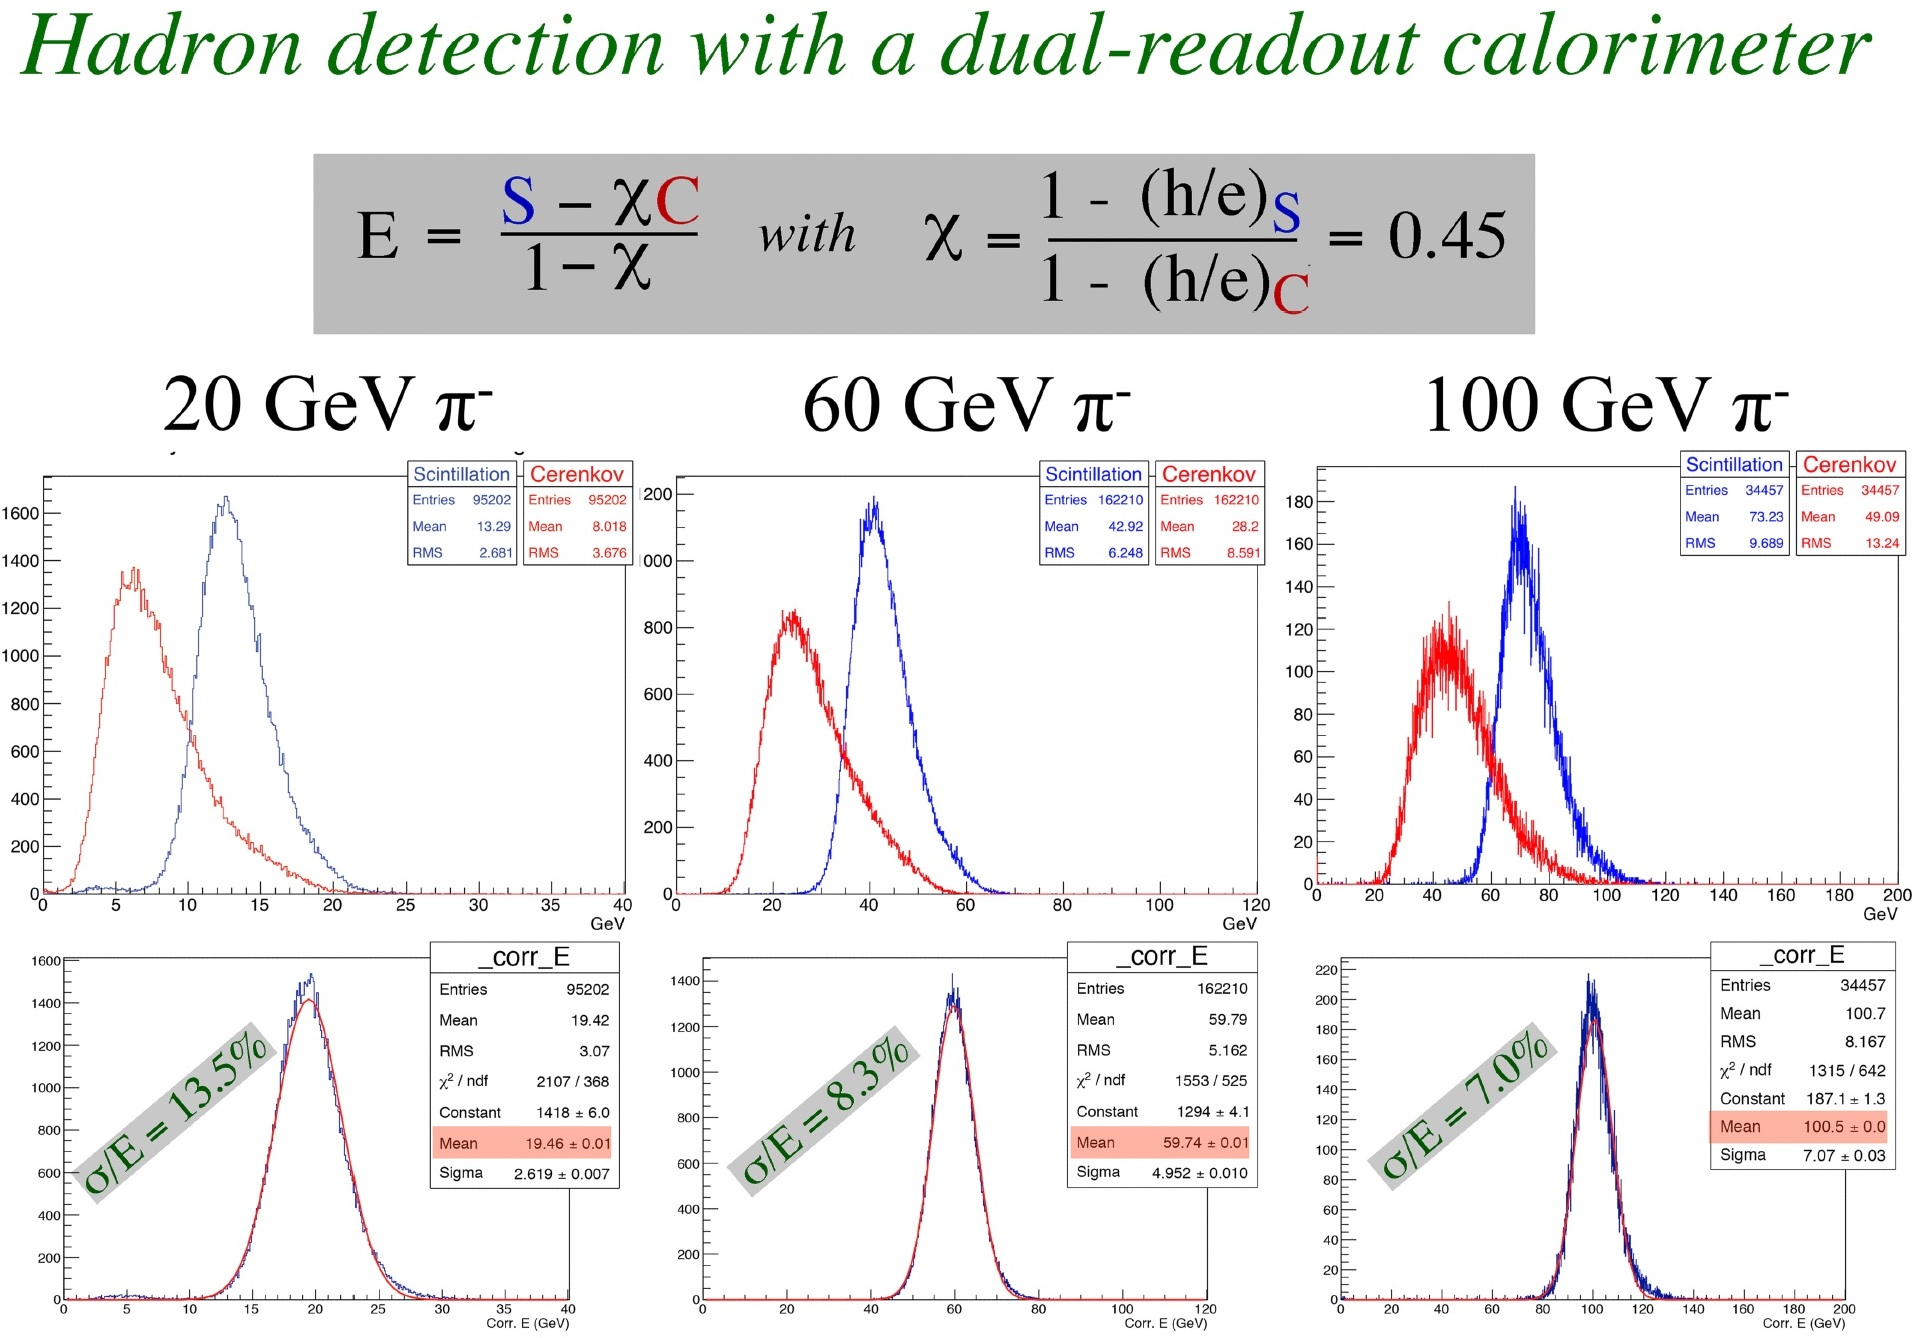
\includegraphics[width=\linewidth]{Calorimeter/DualReadout/Res-pion-20-60-100GeV.jpg}
\caption{Raw scintillation and Cerenkov data for 20, 60, and 100 GeV pion beam, and the dual readout response below}
\label{fig:DualReadout:PionResponse}
\end{figure}

About 30 dual-readout papers are published in Nucl. Intrs. Meths., Rev. Sci. Instr., and JINST, including dual-readout in several crystals, a planar geometry, as well as fibers in several geometries.
We have built and tested Pb-based and Cu-based dual-readout modules and are designing a W-based test module. Typical readout of the Pb-modules is shown in Figure~\ref{fig:DualReadout:PionResponse} for 20, 60, and 100 GeV pion beams in the H8 beam of the North Area at CERN.
Simple dual-readout yields a Gaussian and linear response, currently limited by lateral leakage fluctuations in the Pb-based modules of about 1 tonne.
The record holder for linear, Gaussian energy resolution is still the SPACAL module of 20 years ago, built by Wigmans at CERN to demonstrate the newly understood
concept of ``compensation''. SPACAL was a Pb-scintillating fiber module of mass
20 tonnes that collected scintillation light for 100-200 ns to achieve compensation
from the np $\to$ np recoils in the scintillating fibers. We show in Fig. 2 the hadronic
energy resolutions for single pions for SPACAL, DREAM, and the new RD52 modules, plotted vs. $1/\sqrt{E}$, so that the slope is the stochastic term and the intercept is the constant term.
\begin{figure}
	\centering
	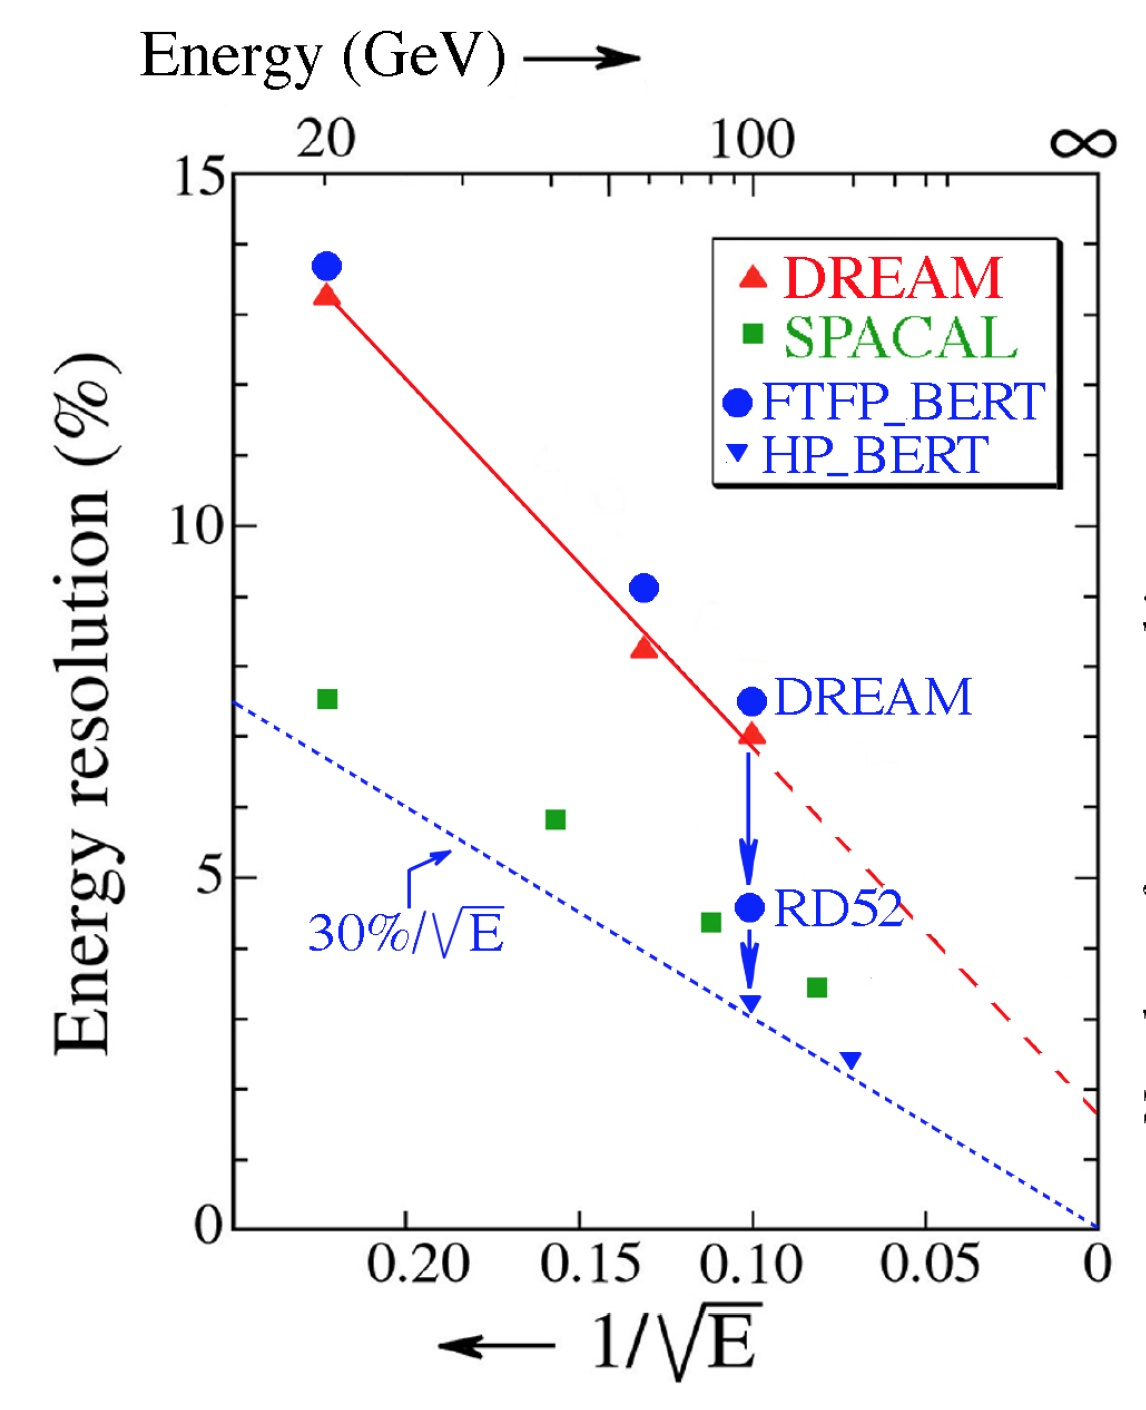
\includegraphics[width=.5\textwidth]{Calorimeter/DualReadout/Eres}
	\caption{The Gaussian-fitted energy resolution of compensating and dual-readout fiber calorimeters. The RD52 copper-fiber dual readout energy resolutions at \unit[100]{GeV} and \unit[200]{GeV} energies for incident pions are shown as the inverted blue diamonds with the label caption \texttt{HP\_BERT}. The dotted line is a resolution of $\sigma/E = 30\%/\sqrt{E}$ with zero constant term. The grant result seems to have a constant term of about 0.5\%.}
	\label{fig:DualReadout:PionResolution}
\end{figure}
A calorimeter with the ILC goal for hadronic energy resolution of
$\sigma/E = 30\%/\sqrt{E}$
is shown as the thin red line. We have not yet achieved this goal, but we know we are limited merely by lateral leakage fluctuations which can be suppressed by a larger module. As shown in Fig. 2 we are closing in.
There are several improvements over the results in Figure~\ref{fig:DualReadout:PionResolution} for (a) Cerenkov photoelectron yield, (b) photocathode efficiency, (c) fiber quality, (d) optical uniformity and, finally, (e) absorber mass. All of these are planned for testing one year from now at CERN. We expect,
based on our data, simulations, and our understanding, that we are likely to achieve a resolution of about $30\%/\sqrt{E}$ with a small constant term. This would result in 3\% energy resolution at 100 GeV and about 2\% energy resolution at the highest SPS beam energies available at CERN.
\begin{figure}
	\centering
	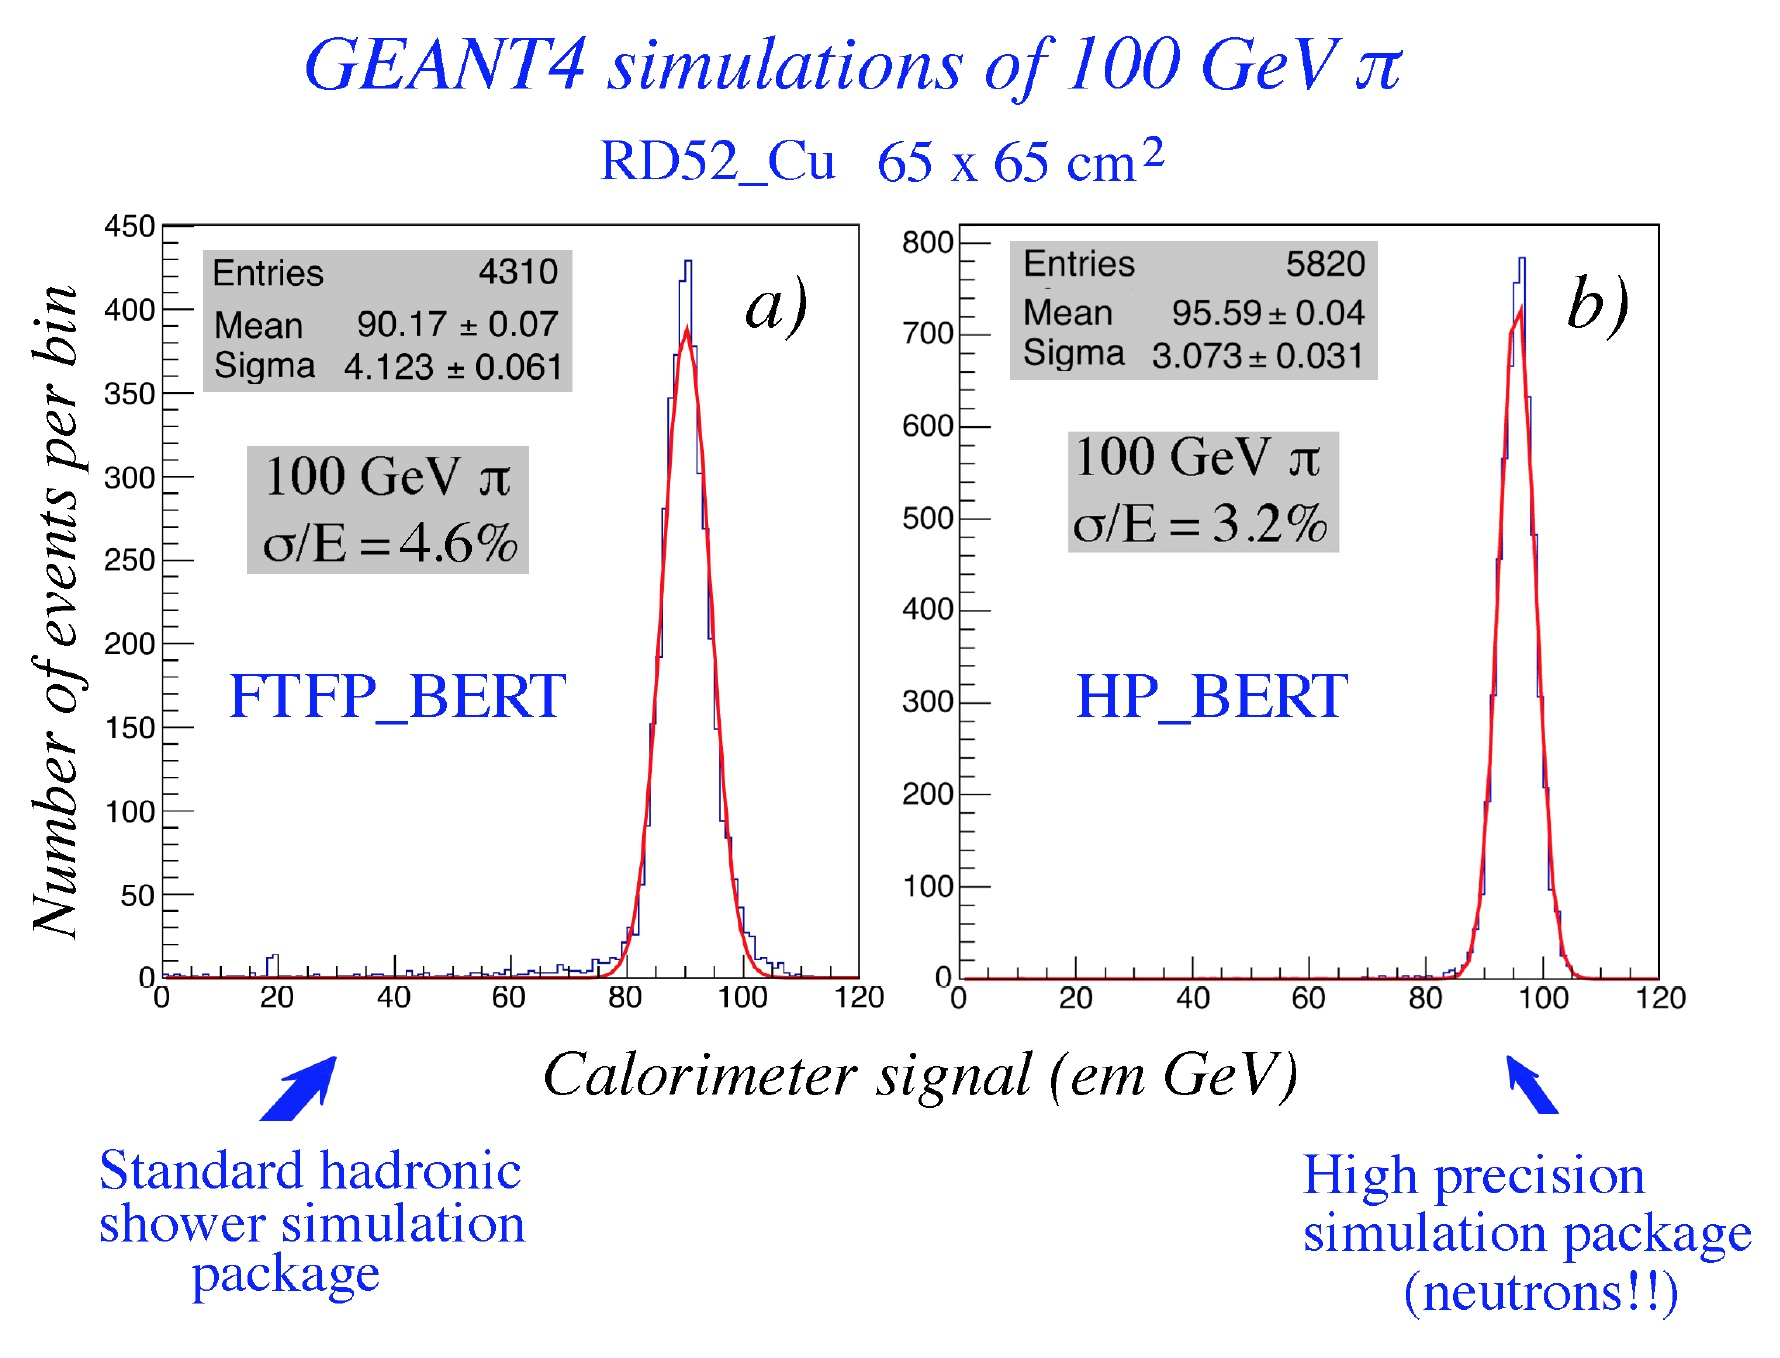
\includegraphics[width=.5\textwidth]{Calorimeter/DualReadout/pi-100GeV-geant}
	\caption{The raw pulse height distribution simulated from two \texttt{GEANT4} physics lists. The latter one does a more correct treatment of the neutrons in the hadronic cascade and, therefore, better represents the dual-readout response of a hadronic calorimeter. Left: Standard hadronic shower simulation. Right: High precision hadronic shower simulation.}
	\label{fig:DualReadout:PionResolutionNew}
\end{figure}
\subsection{Engineering Challenges}
Manufacturing of the high-precision absorber, whether Pb or Cu or W. Assembly of a large calorimeter involves a lot of fibers which can and must be automated. Control of the optics to 1\% is a challenge. It should be emphasized that we do not have engineers working on RD52, but rather find simple solutions which achieve the physics goals without expending large funds. On a construction project, engineering design would improve all our results.
\subsection{Future Plans}
Solving the problems of projective geometry; implementation of SiPM readout; manufacture of a tungsten W-absorber with full dual-readout capability; test of a gaseous dual-readout calorimeter.
\subsection{Applications Outside of Linear Colliders}
High precision calorimetry is vital to many experiments, both collider and fixed target; dual-readout is considered for a space station experiment; and, a high-precision dual-readout calorimeter is being considered for an electron -- ion collider.
\subsection{References}
Complete papers, figures, proposals, status reports, and photos are accessible at our website: http://highenergy.phys.ttu.edu/dream/.
